%%%%%%%%%%%%%%%%%%%%%%%%%%%%%%%%%%%%%%%%%%%%%%%%%%%%%%%%%%%%%%%%%%%%%%%%%%%%%%%%%%%%%%%%%%%%%%%%%%%%%%%
%%%%%%%%%%%%%% Template de Artigo Adaptado para Trabalho de Diplomação do ICEI %%%%%%%%%%%%%%%%%%%%%%%%
%% codificação UTF-8 - Abntex - Latex -  							     %%
%% Autor:    Fábio Leandro Rodrigues Cordeiro  (fabioleandro@pucminas.br)                            %% 
%% Co-autor: Prof. João Paulo Domingos Silva  e Harison da Silva                                     %%
%% Revisores normas NBR (Padrão PUC Minas): Helenice Rego Cunha e Prof. Theldo Cruz                  %%
%% Versão: 1.0     13 de março 2014                                                                  %%
%%%%%%%%%%%%%%%%%%%%%%%%%%%%%%%%%%%%%%%%%%%%%%%%%%%%%%%%%%%%%%%%%%%%%%%%%%%%%%%%%%%%%%%%%%%%%%%%%%%%%%%
\section{\esp Introdução}


O uso de PACS(\textit{Picture Archiving and Communication System}) tem se expandido em todo o mundo \cite{REF08}. A partir de sua utilização, torna-se possível armazenar, compartilhar, recuperar e auxiliar o diagnóstico através de imagens médicas. 
Uma de suas maiores vantagens é o uso desses sistemas para possibilitar, a um paciente, o acesso a um especialista que não esteja próximo fisicamente. 
Hoje é possível fornecer a análise de uma imagem médica, feita por especialistas de forma remota, em lugares onde haja sua carência e necessidade. \cite{REF01} \cite{REF04}.

Os PACS foram criados no decorrer da evolução da Telemedicina. 
Esta tem como objetivo explorar os problemas que envolvem a área da medicina com auxílio da tecnologia.
Consiste essencialmente da informação compartilhada e disponibilizada entre pelo menos dois locais física e geograficamente separados, para fins educacionais ou de saúde \cite{REF01}. 
Com o seu uso torna-se possível capturar, armazenar, transmitir e até mesmo melhorar a informação na forma de registros clínicos, sons, imagens estáticas e vídeos \cite{REF12}.

O termo PACS consiste em uma tecnologia que prove o armazenamento econômico e acesso conveniente a imagens médicas de múltiplas modalidades \cite{REF11}. O uso desses sistemas beneficiam todas as partes envolvidas, tanto pacientes quanto médicos.
Entre alguns dos benefícios estão: o acesso a especialistas de forma remota, compartilhamento de dados clínicos e imagens, economia na não impressão do filme radiológico (formato digital) e custos relacionados a transporte e deslocamento.
Apesar dos benefícios e grande aceitação por parte de seus usuários, existem fatores que devem ser explorados para que seu uso seja eficiente e satisfatório.

No Brasil, as capitais geralmente são dotadas de grandes centros de saúde e avançados equipamentos para geração de imagem médica de diferentes modalidades.
A capital ainda detém uma maior concentração de especialistas médicos, facilitando assim, o processo do diagnóstico.
Em contrapartida, os centros de saúde de cidades mais afastadas das capitais tendem a não ter a mesma proporção de especialistas.
Em sua grande parte, esses centros têm a presença dos equipamentos, mas não dispõem de um profissional para trabalhar com o diagnóstico a partir da imagem.

A falta de investimento e estrutura também é um dificultador, pois um PACS deve ser acessível e estável na grande maioria do seu tempo.
Por exemplo, um médico localizado no interior de seu estado deseja consultar exemplos de anomalias genéticas.
Esse profissional deve ter a garantia que haja uma estrutura adequada na sua instituição para acesso ao sistema.
Da mesma forma, o sistema deve fornecer o acesso remoto rápido e conveniente aos seus serviços, de forma segura e estável, com o mínimo possível de indisponibilidade de acesso \cite{REF19}.

Os terminais de utilização do sistema devem ter acesso a uma grande base de dados de imagens, através do acesso remoto.
Esse acesso deve ocorrer de forma eficiente, segura e flexível, aceitando imagens médicas de múltiplas modalidades \cite{REF18}.
Para isso, as imagens devem possuir uma série de requisitos para auxiliar no diagnóstico médico.
É também necessário ser estabelecido uma estratégia para o armazenamento da imagem, uma vez que a imagem médica é composta de uma imagem propriamente e metadados.
Isso gera uma preocupação com o espaço a ser disponibilizado no disco para armazenamento de todas essas informações \cite{REF10}.

As ferramentas de PACS têm como principal fonte de dados as imagens, que podem ser de uma ou múltiplas modalidades.
Torna-se então essencial definir diretivas para a entrada e saída de dados no sistema.
Caso os dados não atendam a essas diretivas, o material acaba não contribuindo para o estudo ou pesquisa, tornando-se obsoleto.
As PACS atuais implementam essas diretivas através do DICOM, um protocolo criado com o objetivo de normalizar a formatação, envio e recuperação de imagens médicas \cite{REF20}.
Ele permite que suas informações sejam transmitidas entre equipamentos responsáveis por gerar a imagem, terminais de auxílio ao diagnóstico, médicos e hospitais. 

Na Figura \ref{fig:figura1} é possível visualizar a arquitetura de um PACS remoto. O fluxo se origina no envio de registros clínicos de forma remota a central de dados do sistema. Posteriormente o especialista médico faz o acesso a um terminal para a solicitação desses registros. O terminal então consulta a central de dados remota. A central irá realizar o devido tratamento dos dados e retornará a informação solicitada pelo especialista.

% Figura
\begin{figure}[ht]
	\centering	
	\caption[\hspace{0.1cm}Diagrama da Arquitetura.]{Representação de um PACS remoto}
	\vspace{-0.4cm}
	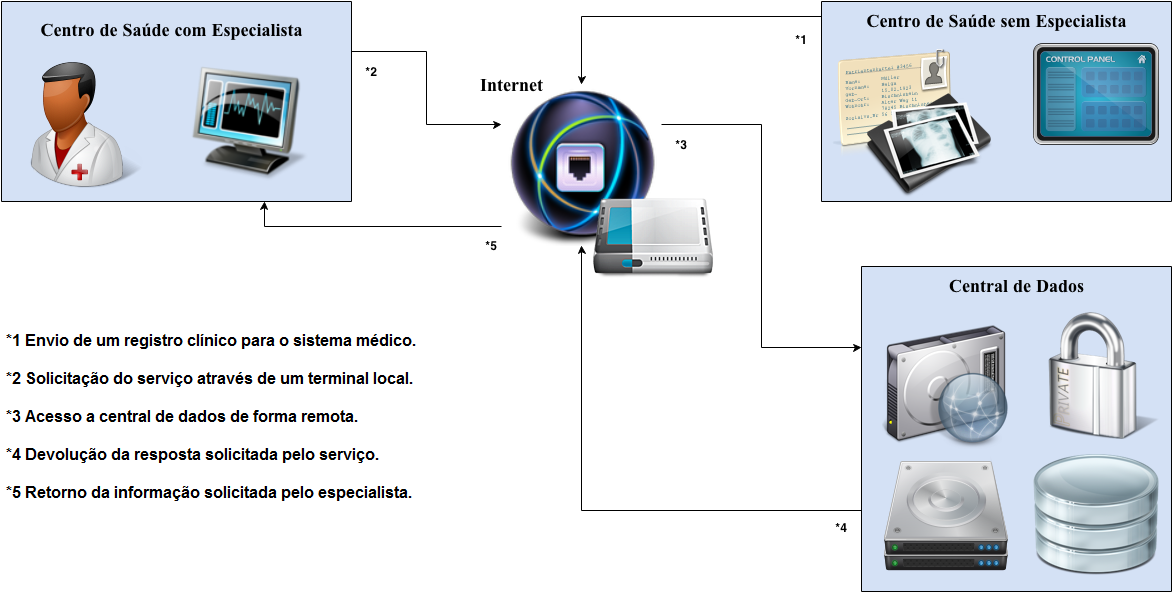
\includegraphics[width=1.0\textwidth]{figuras/diagramas/remoto.png}
	% Caption centralizada
	% 	\captionsetup{justification=centering}
	% Caption e fonte 
	\vspace{-0.2cm}
	\\\textbf{\footnotesize Fonte: Autoria Própria }
	\label{fig:figura1}
\end{figure}

Obedecendo aos requisitos de forma adequada, é possível suprir a grande necessidade de uma base de dados remota para auxílio ao diagnóstico médico.
Deve ser disponibilizado para o paciente um diagnóstico ágil e preciso, devido à quantidade e versatilidade de dados fornecidos pelo sistema.
Além disso, com sua devida utilização e crescimento, o sistema possuirá uma base de dados sólida e confiável para o estudo da Medicina, possibilitando a pesquisa de casos e criando-se um centro para estudo desses materiais.

Para o desenvolvimento de um sistema que atenda a essas características, várias áreas da Computação precisam ser envolvidas.
É necessário o planejamento da forma que as imagens médicas serão armazenadas e recuperadas pelo sistema, criando-se a necessidade do estudo de um banco de dados adequado para a aplicação, assim como a escolha de um sistema de arquivos que favoreça seu funcionamento.
É necessário também o uso de redes de computadores, para a correta disponibilização de um sistema remoto estável.

Um outro aspecto importante é a segurança do sistema. Esta deve ser planejada de forma que a inserção e recuperação de toda essa informação ocorra de forma adequada, eficiente e confiável.
O acesso deve ser fornecido apenas para usuários autorizados e com fins de pesquisa, educacionais ou auxílio ao diagnóstico.

Este trabalho objetiva propor uma ferramenta para o armazenamento, recuperação e apoio ao diagnóstico através de imagens médicas.
A ferramenta pretende auxiliar diversas instituições, profissionais e centros de saúde de forma remota, a juntos criarem uma base de dados compartilhada para consulta e armazenamento de imagens, auxiliando no estudo e pesquisa de áreas como a medicina, telemedicina e ciência da computação.

A ferramenta será hospedada no Hospital das Clínicas da UFMG.
Em uma primeira fase, o sistema irá se destinar ao apoio diagnóstico médico através de imagens radiológicas de anomalias genéticas.
Os usuários serão divididos em grupos de acordo com seu papel no sistema, sendo compostos por: funcionários, médicos, pessoal autorizado do hospital e se necessário, usuários externos.

\section{\esp Referencial Teórico}


As soluções disponibilizadas pela Telemedicina tornam possível capturar, armazenar, transmitir e até mesmo melhorar a informação na forma de registros clínicos, sons, imagens estáticas e vídeos \cite{REF02}.
Sua área e subáreas trazem benefícios para médicos, hospitais e instituições, além do paciente, seu maior beneficiado.
De acordo com \cite{REF04}, os mais beneficiados através das ferramentas de Telemedicina são os consumidores.
A partir de sua utilização é possível levar um atendimento de qualidade, acessível e de baixo custo para o paciente.
Como empresas de saúde já estão mostrando, é possível trazer saúde ao ponto de necessidade, não sendo necessário transportar o paciente a um ponto de atendimento de difícil acesso.

Mesmo com seus benefícios, desde o surgimento do termo de Telemedicina até os dias atuais, a literatura mostrou que, apesar da grande evolução tecnológica, muitos desses sistemas não conseguem manter-se ou prolongar sua existência \cite{REF16}.
Fatores como a resistência e falta de treinamento de profissionais são citadas como grandes barreiras para impedir sua sustentabilidade e progresso \cite{REF03}.
A implementação dessa tecnologia requer mudança e treinamento de seus envolvidos.
Processos de pequeno nível, como disponibilização de suporte e treinamento para profissionais e pacientes mostram-se necessários, enquanto um maior nível de amadurecimento é requisitado em instituições de cuidados a saúde \cite{REF06}.

Tendo em vista essas dificuldades surgiram estudos com o objetivo de entender os problemas apresentados na implementação e integração desses sistemas.
Revisões literárias como a proposta por \cite{REF02} procuram apresentar o motivo de falha ou sucesso do sistema ou mecanismo de comunicação, identificando barreiras e facilidades para futuras implementações.
Apesar desses identificarem os fatores e seus respectivos resultados, os autores não focam na estrutura metodológica utilizada durante o processo, tornando-se difícil para quem procura desenvolver um sistema com essas características encontrar conceitos genéricos e aplicáveis para a implementação \cite{REF09}.

Um PACS consiste em uma tecnologia médica que forneça armazenamento econômico e acesso conveniente de imagens médicas de múltiplas modalidades (tipos de máquinas de origem diferentes).
A intenção desse sistema é substituir os filmes radiográficos, armazenando a imagem de forma digital, devido às vantagens na relação custo/benefício em comparação ao antigo armazenamento em filme \cite{REF13}.
Pela imagem digital é possível realizar a distribuição e acesso remoto dos registros clínicos por especialistas da saúde.
Isso torna o processo de diagnóstico médico veloz e, se unido à aplicação de certo processamento na imagem, pode auxiliar a recuperação ou melhorar a disponibilização de informações nela contidas \cite{REF05}.

Um PACS que se proponha a recuperar e compartilhar imagens deve atender requisitos mínimos em diversos aspectos \cite{REF03}.
Um desses aspectos é a disponibilidade do sistema.
O sistema irá atender a médicos e pacientes, logo deve estar disponível durante o maior tempo possível.
Dados coletados por \cite{REF19} mostram que 20\% dos seus usuários encontraram o sistema indisponível mais de sete vezes no ano.
Pode parecer um número pequeno, mas tratando-se de um sistema de saúde, este dado é alarmante.
Em média, um sistema de saúde fica indisponível quatro dias em um período de um ano e seis meses.

IRMA (\textit{Image Retrieval in Medical Applications}) é um sistema para recuperação de imagens médicas. Esse sistema torna possível a procura e recuperação de registros clínicos através de um banco de dados extenso de imagens digitais.
A maneira mais comum de recuperar essas imagens é a inserção de suas informações em forma textual seguido de sua busca no banco de dados \cite{REF08}.
Hoje em dia, a maioria dos PACS faz uso apenas de informações textuais, como dados clínicos do paciente, para a recuperação da imagem médica \cite{REF04}.
Esses sistemas devem conter a possibilidade de armazenamento das características das imagens, para que a recuperação possa ser feita não apenas com as informações e registros do paciente, mas também através de imagens semelhantes \cite{REF10}.

Contudo, a qualidade dessas imagens deve atender o uso de sua aplicação.
Sistemas de imagens médicas trabalham com a recuperação da imagem e sua distribuição para os médicos.
Estes precisam ter uma imagem adequada para que possam realizar estudos e para que o próprio sistema possa realizar algum tipo de processamento, destacando alguma informação que seja de interesse \cite{REF12}.
Uma imagem que não tenha boa qualidade poderá atrapalhar um possível diagnóstico do profissional \cite{REF07} \cite{REF15}.

Os sistemas baseados em recuperação de imagens de propósito geral geralmente programam extração, armazenamento e comparação de características, além de uma interface para a recuperação da imagem \cite{REF18}.
Apesar desses sistemas oferecerem um grande número de rotinas para extração e comparação, eles pecam na não organização das características armazenadas.
\cite{REF10} propõem a utilização de um framework para desenvolvimento e implantação de sistemas baseados em recuperação de imagens médicas, que deixa o uso desses sistemas acessível para o usuário final, sem que este precise saber dos detalhes técnicos dos métodos para utilização.
Dentre os fatores mais importantes para o desenvolvimento de um sistema para recuperação de imagens médicas estão a flexibilidade e extensibilidade do sistema \cite{REF18}.
No artigo de \cite{REF10}, foi proposto um modelo de arquitetura para o desenvolvimento de sistemas com essas características.

A plataforma apresentada por \cite{REF18} é dividida em camadas genéricas para um conjunto de operações.
Cada uma delas é responsável por fornecer, à camada superior ou inferior, uma entrada e saída.
A camada superior consiste de um site desenvolvido em PHP.
Esse site se comunica com um uma camada mais baixa, que consiste em um WebService JAVA, que retorna respostas de formato XML ou JSON.
Ainda no WebService, está presente o Banco de Dados e o sistema de arquivos.
Mais abaixo temos a camada de processamento da imagem, que utiliza de algoritmos desenvolvidos em C++ para a extração de características e a recuperação da imagem por conteúdo.

A primeira camada fornece interfaces ao usuário para realizar suas operações: basicamente o fornecimento de uma nova imagem médica para o sistema, e a recuperação de uma imagem através de suas informações textuais.
Após a seleção da operação e do fornecimento dos dados, o site se comunica com o WebService Java. Este é caracterizado pelo controle de requisições e respostas solicitados pelo site.
Nesta camada são tratadas as operações de inserção ou recuperação de imagens.
O serviço retorna respostas XML ou JSON as solicitações realizadas pelos usuários.
Nesta camada ocorre a comunicação com o banco de dados, que retorna as informações da imagem e seu caminho de acesso no sistema de arquivos.

Com relação à camada de processamento, a inserção de uma imagem utiliza a extração de suas características, que podem ser de três tipos: transformação de várias características em um a(T:1), transformação de uma característica em uma (1:1), transformação de uma característica em um conjunto de características (1:T)\cite{REF10}.
Já na busca por uma imagem, essa camada será responsável pela aplicação de algoritmos desenvolvidos em C ou C++ que proponham a recuperação de uma imagem utilizando seu conteúdo visual.

A arquitetura necessita ser extensível, permitindo ao desenvolvedor anexar futuros algoritmos para processar a imagem de diferentes formas.
Como dito em \cite{REF18}, esses sistemas devem ser capazes de permitir a extensão e flexibilidade das formas de recuperação e armazenamento das imagens.
Para isso são utilizados arquivos XML, que determinam as propriedades das interfaces e parâmetros adicionais, de cada algoritmo de processamento de imagens.

\section{\esp Metodologia}


O sistema foi implementado de acordo com a arquitetura sugerida por \cite{REF10}.
A primeira camada implementada foi o site. Esta conta com várias interfaces que possibilitam ao médico ou ao usuário responsável o envio de informações ao WebService.
Como dito em \cite{REF09}, um dos problemas que dificultam o uso dessas tecnologias é a resistência do profissional a novas ferramentas.
Para mudar esse paradigma, as interfaces fornecidas pelo sistema devem ser cuidadosamente planejadas.
Fatores como acessibilidade, flexibilidade e interatividade devem ser explorados.

Para atender aos requisitos de uma interface intuitiva e clara foi utilizado o Java Server Pages (JSP).
Este integrado ao HTML, permite adicionar dinamismo a páginas web, criando padrões e reutilizando componentes nas interfaces.
Para oferecer um padrão visual e acessível aos componentes do JSP, as interfaces foram desenvolvidas através da utilização do \textit{framework} Bootstrap.
Enquanto o JSP se preocupa com a estruturação do  documento, o \textit{framework} reúne uma série de recursos que contribuem com o visual da interface. Também foi utilizado o \textit{framework} jQuery, com propósito de auxiliar em uma melhor interação do usuário e interface.

A primeira camada também oferece suporte para a visualização de imagens médicas através do navegador Web. Esta ferramenta foi desenvolvida com auxílio dos \textit{frameworks} citados anteriormente. A biblioteca manipula uma imagem JPEG através do elemento \textit{Canvas}, um recurso oferecidos pelo HTML5 que permite a manipulação de imagens em um documento Web. Ela fornece ao médico uma interface dinâmica para a visualização de registros clínicos de determinado paciente. Para imagens médicas é possível aplicar operações que facilitem o diagnóstico. A biblioteca ainda permite que outros algoritmos de processamento de imagens possam ser futuramente anexados e utilizados.

A interface do sistema necessita do WebService para seu correto funcionamento. Porém, o serviço Web não necessita da interface para realizar suas operações. Ele foi implementado de forma que possa interagir com outros sistemas, manipulando requisições HTTP padronizadas.
O processo de comunicação se resume no seguinte fluxo: um usuário através de uma interface (essa pode ser um sistema ou mesmo um terminal) realiza solicitações, que são gerenciadas pelo serviço Web.
Uma requisição HTTP é enviada para o servidor responsável pelo serviço Web, na tentativa de uma possível inserção ou busca de dados e imagens médicas.
Ao término do processamento da requisição no servidor uma resposta é retornada, esse retorno pode indicar sucesso ou falha da operação.

Assim como a arquitetura proposta por \cite{REF10} o serviço Web tem como formato de suas respostas os padrões XML ou JSON.
Ambos são padrões universais de intercâmbio de dados. Como o âmbito do sistema é ser flexível, os dois formatos foram adotados como tipo de resposta as requisições.
O XML (\textit{Extensible Markup Language}) é uma linguagem de marcação, amplamente utilizada no intercâmbio de dados entre sistemas.
O JSON (\textit{Javascript Object Notation}), como seu nome diz, é a notação de um objeto na linguagem JavaScript e assim como o XML, também é utilizado para tráfego de dados.
Os dois possuem vantagens e desvantagens, porém esses pontos não serão abordados. O objetivo aqui é oferecer uma arquitetura flexível \cite{REF18}.

Os dados retornados como resposta às requisições são representações textuais de objetos Java.
Por exemplo, um paciente físico é mapeado no sistema através de uma instância da classe \textit{Paciente}.
A instância da classe será então convertida em uma cadeia de caracteres nos formatos padrões do sistema, JSON ou XML.
Para realizar essa conversão, foi necessário a utilização de duas bibliotecas de \textit{parser}.
A Google Data APIs Cliente Library é uma delas, responsável por converter um objeto na linguagem Java para um \textit{String} textual no formato XML.
A Google-JSON API foi a outra biblioteca utilizada, que faz semelhante conversão, porém tem como retorno uma \textit{String} JSON.

Após o tratamento dos dados recebidos pela requisição HTTP, o serviço WEB deve gerenciar todo o fluxo de operações internas. Esse estágio consiste na comunicação com o sistema de arquivos e banco de dados.
O modelo de arquitetura em camadas também foi adotado no desenvolvimento do WebService. Ele foi planejado e implementado baseado no conceito Modelo-Visão-Controlador (MVC) \cite{REF21}.
O MVC é um modelo de arquitetura de software que separa a interação do usuário com dada interface da representação e do armazenamento da informação. Na Figura \ref{fig:figura2} é possível visualizar a arquitetura adotada para a implementação do serviço Web.

\begin{figure}[ht]
	\centering	
	\caption[\hspace{0.1cm}Diagrama de Sequência.]{Diagrama de sequência da Arquitetura}
	\vspace{-0.4cm}
	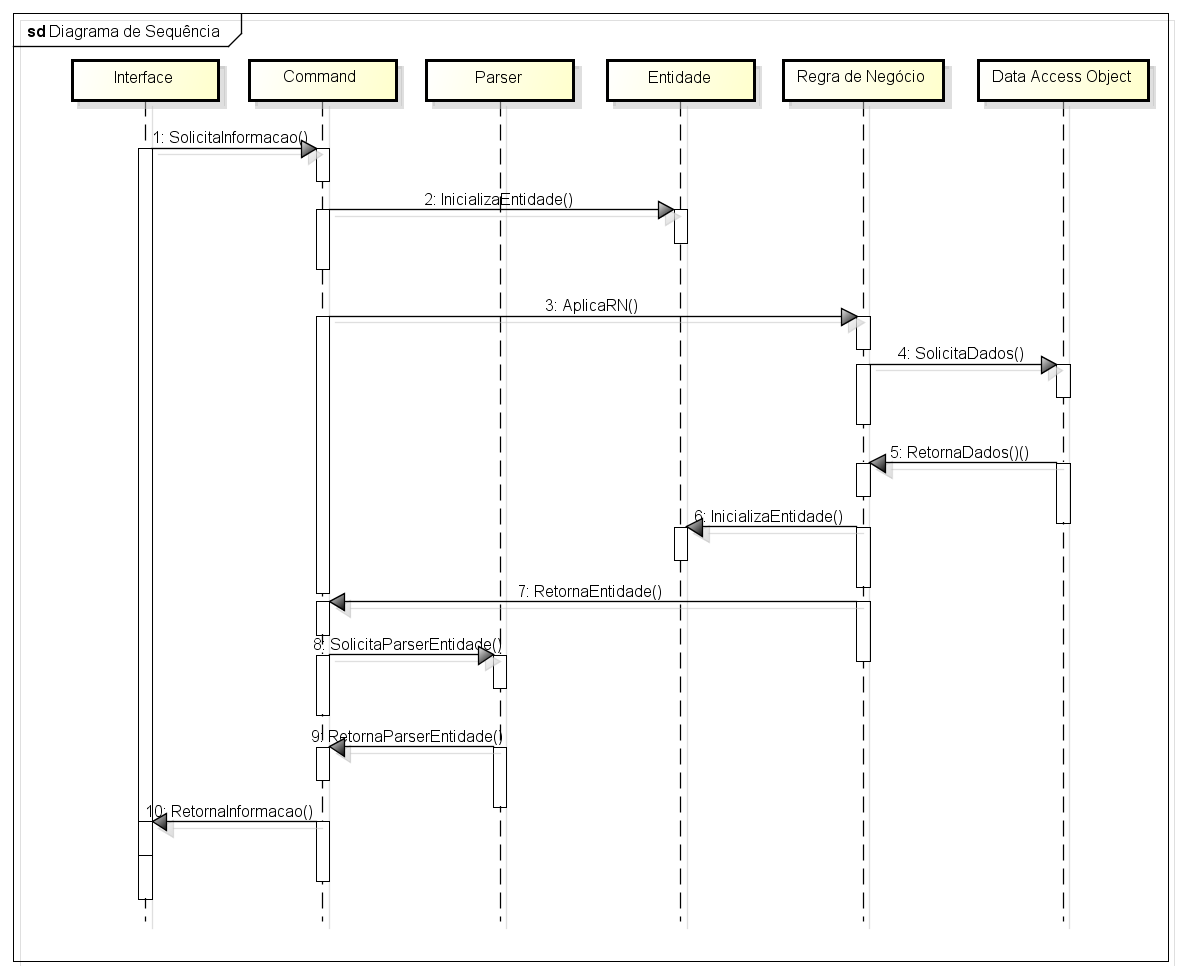
\includegraphics[width=1.0\textwidth]{figuras/diagramas/sequencia.png}
	% Caption centralizada
	% 	\captionsetup{justification=centering}
	% Caption e fonte 
	\vspace{-0.2cm}
	\\\textbf{\footnotesize Fonte: Autoria Própria }
	\label{fig:figura2}
\end{figure}

Para implementação do serviço de acordo com este modelo, foi projetado um controlador de fluxo.
O controlador gerencia todas as requisições enviadas por usuários do sistema.
Por exemplo, quando um usuário solicita a busca por uma imagem radiológica, a primeira tarefa é avisar ao serviço qual a operação deve ser executada.
Para esta designação de tarefas foi utilizado um \textit{Servlet}, tecnologia Java utilizada para estender as funções de um servidor.

Quando uma tarefa é designada pelo controlador, o serviço realiza um redirecionamento no fluxo.
O fluxo então é continuado através de um classe do tipo command (\textit{CMD}).
O \textit{CMD} também utiliza a tecnologia \textit{Servlet}, mas seu escopo está limitado a apenas uma operação.
As ações dessa classe se resumem em transformar os dados fornecidos pelo controlador em informações.
Essas serão transmitidas para as classes de regra de negócio, comunicação com o banco de dados e sistema de arquivos.
Um exemplo disso seria o gerenciamento do armazenamento de todas as novas imagens que um usuário deseja inserir no banco de dados e sistema de arquivos.

As classes responsáveis pela regra de negócio (\textit{RN}) contem uma série de diretivas e políticas necessárias para que uma operação seja realizada.
No exemplo anterior, em que foi citada a operação de armazenamento de uma nova imagem, uma regra de negócio seria controlar se a imagem radiológica está adequada aos formatos aceitos pelo sistema.
Essas classes são geralmente utilizadas antes ou após uma operação no banco de dados ou no sistema de arquivos.

Para a comunicação com o banco de dados foi utilizado o Hibernate, um \textit{framework} Java para persistência dos objetos da linguagem e seu mapeamento no banco de dados.
A persistência é feita através do mapeamento de uma classe Java com uma tabela no banco de dados, utilizando o modelo relacional.
A implementação desse modelo é auxiliada pelo uso de duas classes. Uma classe Business Object (\textit{BO}) e uma Data Access Objet (\textit{DAO}).
As classes \textit{BO} são o mapeamento de uma entidade em uma tabela do banco de dados, e as classes \textit{DAO} são responsáveis por detalhar e construir as consultas (SQL) a se serem realizadas.
Por exemplo, um registro clínico do sistema seria representado por uma classe \textit{BO}, e a forma que esse registro será recuperado no banco de dados é manipulada pela sua classe \textit{DAO}.

Existem ações em que se faz necessário o acesso ao sistema de arquivos.
Por exemplo, quando um usuário deseja recuperar imagens de anomalias genéticas de uma criança.
Terminada a sequência de operações até a recuperação de registros no banco de dados, o sistema terá que se comunicar com o sistema de arquivos.
O motivo da comunicação é o fato das imagens não serem gravadas no banco de dados. O banco contém apenas o caminho físico do sistema de arquivo, onde elas serão gravadas.
Ao final desse processo, a resposta referente à requisição solicitada ao WebService estará pronta para ser entregue.

\section{\esp Resultados}

O sistema foi implementado em uma máquina AMD FX(tm)-4300 Quad-Core, utilizando o sistema operacional Windows 7 de 64bits, Java Runtime environment 1.7, Java Advanced Imaging 1.1.3, e foi testado em um rede ethernet local 100 Mbit/s, utilizando o navegador Web Firefox Developer. As operações foram executadas dez vezes e foi utilizada a média do objeto de estudo para obtenção dos resultados finais. Os testes realizados nesta máquina não apontaram problemas quanto ao tráfego de dados pela rede. Contudo, o intuito do sistema é ser acessado de forma remota e isso gera uma preocupação com a rede disponibilizada para o tráfego das imagens.

Na Figura \ref{fig:figura3} é possível visualizar a interface responsável pelo envio dos registros clínicos de um paciente. Nessa mesma interface foi realizado um teste do envio de múltiplas imagens DICOM simultaneamente. Em média cada imagem levou aproximadamente 0,314s para ser enviada ao sistema de arquivos. O tempo foi medido a partir do momento em que a requisição é recebida no serviço Web. Se houver um grande volume de imagens médicas trafegadas num curto período de tempo, torna-se necessária a disponibilização de uma rede com grande banda destinada para o \textit{upload} de arquivos.

\begin{figure}[ht]
	\centering	
	\caption[\hspace{0.1cm}Imagens Clínicas.]{Solicitação e Envio Imagens}
	\vspace{-0.4cm}
	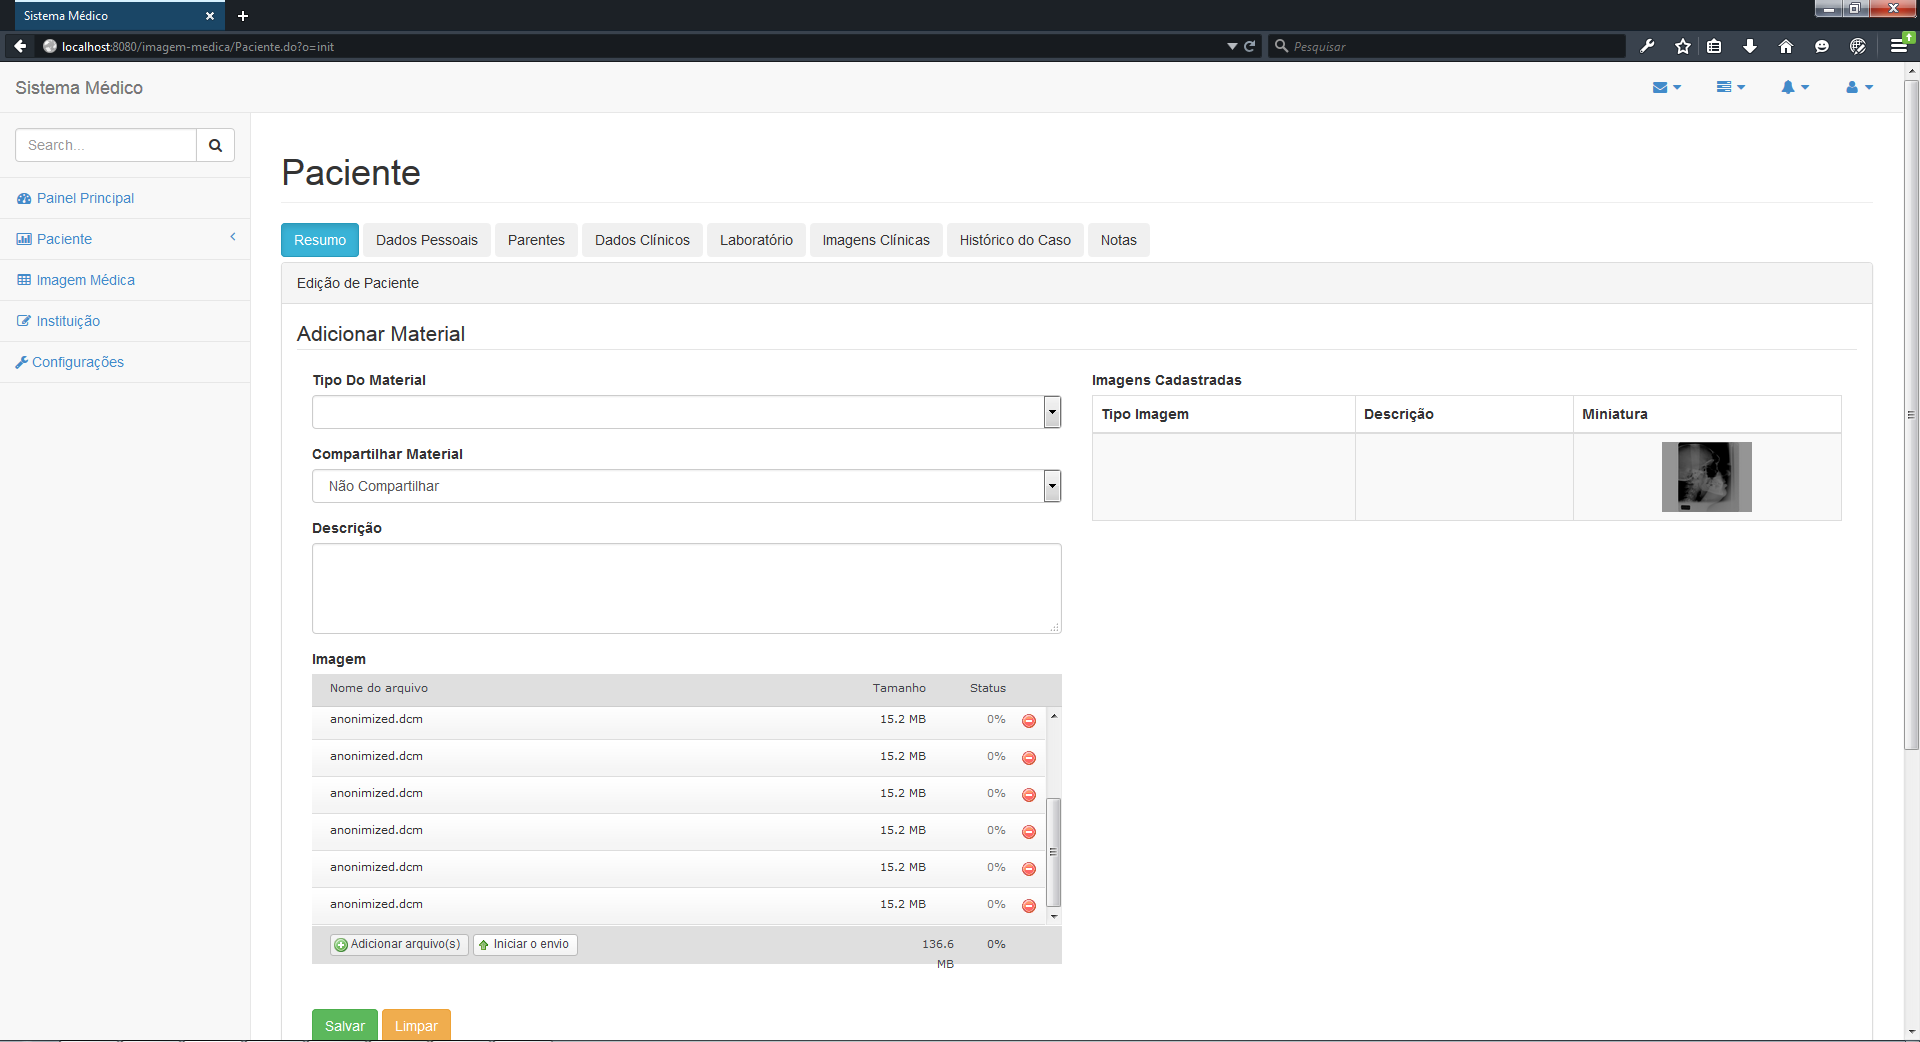
\includegraphics[width=1.0\textwidth]{figuras/envioMultiplasImagens15mb.png}
	% Caption centralizada
	% 	\captionsetup{justification=centering}
	% Caption e fonte 
	\vspace{-0.2cm}
	\\\textbf{\footnotesize Fonte: Autoria Própria }
	\label{fig:figura3}
\end{figure}

A conversão das imagens médicas, quando solicitadas, foi outro ponto observado durante os testes. A interface responsável por gerenciar os registros clínicos do paciente é onde essa solicitação é realizada. Ao se abrir essa interface é feita uma solicitação a cada registro clínico relacionado ao paciente em questão. Cada uma dessas solicitações na máquina testada levou em média 1,180s para ser executada. Nesse tempo está incluso desde a solicitação realizada pelo usuário até o retorno dos dados para o mesmo (incluindo a conversão do formato DICOM para o JPEG). Um sistema com  múltiplos usuários fazendo várias solicitações simultâneas iria necessitar de um bom poder de processamento para realizar essas conversões em tempo hábil. Uma vantagem é que cada solicitação ocorre de forma assíncrona, sem depender do término do processamento de outra imagem. Utilizando essa implementação, o tempo de resposta e carregamento de toda a página diminui consideravelmente.

Um recurso de grande importância para o sistema é a ferramenta para a visualização das imagens. Esta ferramenta para auxílio ao diagnóstico médico é oferecida ao usuário do sistema no próprio navegador Web. Os testes de visualização de imagens foram executados no navegador Firefox Developer. O recurso utilizado para essa visualização é 
oferecido em novas versões dos principais navegadores atuais como Internet Explorer, Firefox, Chrome, Opera e outros. Dessa forma os usuários que desejam fazer o uso do sistema 
para auxílio ao diagnóstico, como médicos e instituições, deverão usar versões atualizadas desses navegadores. O tempo necessário para carregar a imagem na ferramenta é
praticamento nulo (em média 0,001s). Esse custo é baixo devido à prévia solicitação descrita. As imagens são convertidas e retornadas ao site em formato JPEG. Por exemplo, uma  imagem DICOM de 15MB tem como média de tamanho quando convertida para o formato JPEG de 200KB a 300KB. Na Figura \ref{fig:figura4} é possível visualizar a ferramenta acessando uma imagem DICOM através do navegador Firefox.

\begin{figure}[ht]
	\centering	
	\caption[\hspace{0.1cm}Imagens Clínicas.]{Visualização da Imagem Médica}
	\vspace{-0.4cm}
	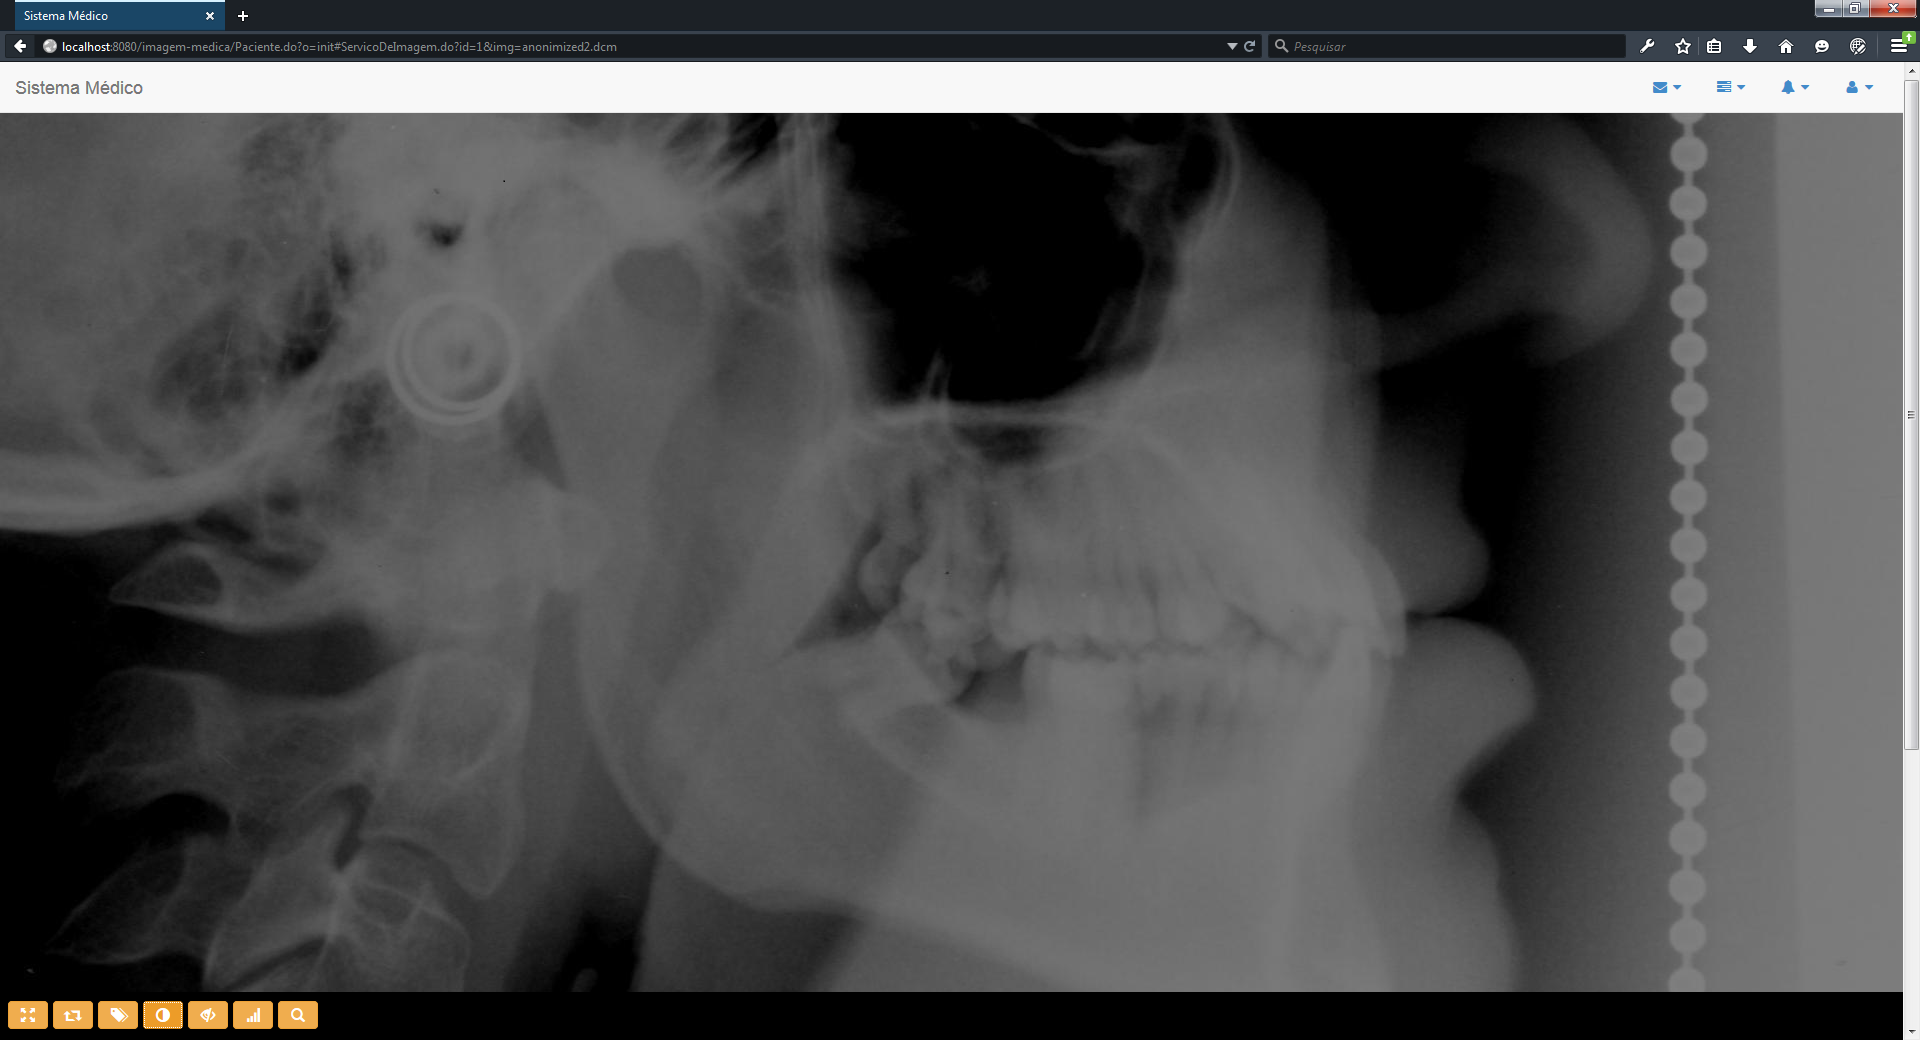
\includegraphics[width=1.0\textwidth]{figuras/visualizacaoImagemMedicaGrandeResolucao.png}
	% Caption centralizada
	% 	\captionsetup{justification=centering}
	% Caption e fonte 
	\vspace{-0.2cm}
	\\\textbf{\footnotesize Fonte: Autoria Própria }
	\label{fig:figura4}
\end{figure}

A ferramenta disponibilizada também oferece métodos básicos de processamento de imagem para o auxílio ao diagnóstico médico. Um exemplo seria a inversão de cores de uma radiografia. Os testes de inversão de cores foram realizados com uma imagem DICOM que foi convertida para o formato JPEG, e após sua conversão tinha como  tamanho 213KB. A inversão de cores dessa imagem através da ferramenta e do navegador Firefox Developer levou aproximadamente 0,238s. 

O acesso e armazenamento das imagens médicas a serem enviadas para o sistema é o ponto mais importante a ser notado. Com o aumento no tráfego de registros clínicos no sistema, um grande espaço para armazenamentos de dados se torna necessário. Por exemplo, se durante um dia forem enviadas ao sistema 30 imagens médicas de aproximadamente 20mb, no período de um mês o sistema já estaria armazenando aproximadamente 17Gb. Torna-se necessário o estudo de novas políticas para o armazenamento desses dados, a forma de acesso e disponibilização além de uma escolha mais criteriosa para um adequado modelo de sistema de arquivos.

O modelo implementado tornou possível a fácil interação entre a interface do sistema e o serviço. Os dados retornados no formato JSON permitem um balanceamento entre as tarefas executadas no servidor e tarefas executadas no cliente (navegador). Na Figura \ref{fig:figura5} temos um gráfico da representação do volume de dados do sistema e o tempo necessário para carregar cada recurso. Um ponto interessante a ser notado é que cada solicitação de imagem médica realizada no servidor é feita de forma assíncrona. As solicitações desta forma permitem que as imagens sejam recuperadas de forma "paralela", sem que uma solicitação espere outra finalizar para ser executada. O processamento de todo o conteúdo da página demorou em média 2,890s, sendo que 0,490s foram destinados a outros recursos. O tempo total para a solicitação das nove imagens de forma assíncrona foi em média 2,400s.


\begin{figure}[ht]
	\centering	
	\caption[\hspace{0.1cm}Imagens Clínicas.]{Tempo Para Carregar os Recursos}
	\vspace{-0.4cm}
	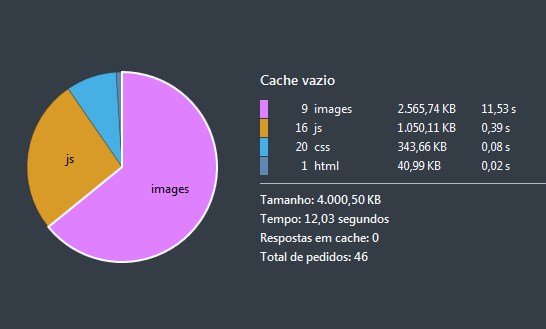
\includegraphics[width=1.0\textwidth]{figuras/analiseTempoIndividualParaCarregarImagens.png}
	% Caption centralizada
	% 	\captionsetup{justification=centering}
	% Caption e fonte 
	\vspace{-0.2cm}
	\\\textbf{\footnotesize Fonte: Autoria Própria }
	\label{fig:figura5}
\end{figure}

\section{\esp Conclusão}

Os resultados após sua implementação mostram trazer uma base para armazenamento e recuperação de imagens médicas de múltiplas modalidades. A ferramenta poderá fornecer à pacientes, centros de saúde e instituições o acesso remoto a um especialista médico. O acesso ao registro clínico na forma digital por esse especialista, agiliza o processo do diagnóstico médico.

O balanceamento de tarefas realizado pela arquitetura é um grande ponto a ser explorado. O processamento das imagens e registros clínicos são realizados no serviço Web, enquanto as ferramentas para auxiliar no diagnóstico médico estão presentes no próprio navegador do usuário. Esse balanceamento permite o controle e estabilidade dos recursos do servidor e das máquinas que acessam o sistema remotamente.

A transmissão de um grande volume de imagens médicas se não tratada de forma eficiente, poderá tornar-se um empecilho para o uso do sistema. Com os resultados obtidos mostra-se necessário o estudo de métodos para o tráfego de arquivos com grande tamanho físico. A demanda por um melhor ambiente de armazenamento e melhores condições na estrutura da rede mostram-se necessárias.

Para trabalhos futuros é interessante o estudo de novas soluções para transmissão dos registros clínicos. A aplicação e estudo de algorítmos para auxiliar a recuperação de imagens médicas também é um ponto interessante a ser explorado. Registros clínicos de uma mesma doença poderão ser equiparados para facilitar ainda mais o processo do diagnóstico médico.


% \subsection{\esp Trabalhos futuros}
% 
% Sugestões de estudos posteriores são ser adicionados subseção deste capítulo de conclusão.
